JUnit tests were used to test this prototype application.
JUnit is a unit testing framework.
Mockito is a framework for JUnit that was also utilised.
Mockito makes mocks of objects for testing.
This is very useful to test database instances as you can mock an SqlLite Database object.

\tocless\subsection{Unit Tests}
\begin{figure}[h]
    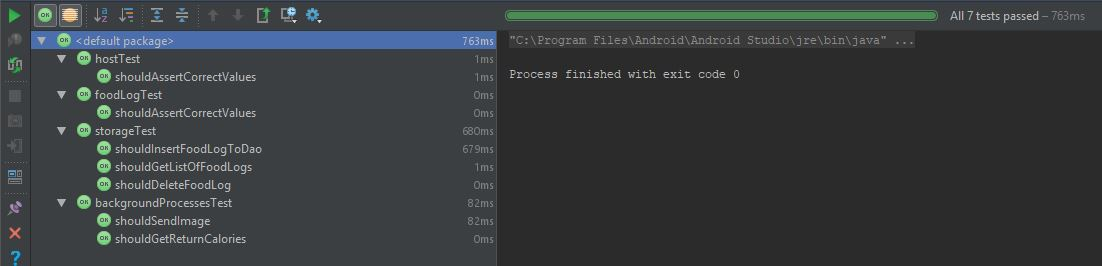
\includegraphics[scale=0.5]{UnitTests}
    \caption{Automated Unit Tests}
    \label{fig:unitTests}
\end{figure}

\tocless\subsubsection{Test to ensure FoodLog object stores information correctly}
\begin{lstlisting}[style=Java]
@Before
public void setUp() {
    foodLog = new FoodLogImpl(0, "banana", 59.03, new Date());
}

@Test
public void shouldAssertCorrectValues() {
    assert food.equals(foodLog.getFood());
    assert calories == foodLog.getCalories();
    assert timestamp.equals(foodLog.getTimestamp());
    assert id == foodLog.getId();
}
\end{lstlisting}

\tocless\subsubsection{Test to ensure Host object stores information correctly}
\begin{lstlisting}[style=Java]
@Before
    public void setUp() {
        host = new Host.HostBuilder("52.214.205.157")
                .withDns("ec2-52-214-205-157.eu-west-1.compute.amazonaws.com")
                .withPort(5000)
                .withRoute("/classifyImage/")
                .build();
    }

@Test
public void shouldAssertCorrectValues() {
    assert this.ip.equals(host.getIpv4());
    assert this.dns.equals(host.getDns());
    assert this.port == host.getPort();
    assert this.route.equals(host.getRoute());
    assert this.urlString.equals(host.getUrl());
}
\end{lstlisting}

\tocless\subsubsection{Test to ensure DAO object stores and removes data correctly}
\begin{lstlisting}[style=Java]
@Before
public void setup() {
    dao = mock(SqlLiteDAO.class);
    date = new Date();
    foodLog = new FoodLogImpl(0, "test", 0.0, date);
}

@Test
public void shouldGetListOfFoodLogs() {
    foodLogs = dao.getLogsByDay(date);
    foodLogs = dao.getLogsByWeek(date);
    foodLogs = dao.getLogsByMonth(date);
}

@Test
public void shouldInsertFoodLogToDao() {
    dao.addFoodLog(foodLog);
    setTestLog();
    assert foodLogs.contains(testLog);
}

@Test
public void shouldDeleteFoodLog() {
    List<FoodLog> foodLogs = new ArrayList<>();
    foodLogs.add(testLog);
    dao.deleteFoodLogs(foodLogs);
    setTestLog();
    assert testLog.equals(null);
}

private void setTestLog() {
    foodLogs = dao.getLogsByDay(date);
    foodLogs.forEach(f -> {
        if(f.getFood().equals("test")) {
            testLog = f;
        }
    });
}
\end{lstlisting}